% !TeX encoding = UTF-8
% !TeX spellcheck = en_GB

%%% Add [final] option to the report class to switch between draft and final version of the report
%%% Use [narrowmargin] to enable narrow margins - this may impair readability.
%\documentclass[a4paper,12pt,draft]{include/intocpsreport}   %Or
\documentclass[a4paper,12pt,final]{include/intocpsassociation}   %Or
% intocpslargereport if chapters are required.
%
%
%
\usepackage[T1]{fontenc}
\usepackage[utf8]{inputenc}
\usepackage{longtable}
\usepackage{tikz-uml}
\usepackage{framed}
\usepackage{subcaption}
\usepackage[hyphenbreaks]{breakurl}
\usepackage{color}
\usepackage{amsmath}
\usepackage{courier}
\usepackage{xspace}
\usepackage{cleveref}
\usepackage{subcaption}
\usepackage{textcomp} % Used for 20-sim section \textrightarrow
%\usepackage{showframe}

\usepackage{listings}
\usepackage{glossaries}

%% Define listing environment for XML
\definecolor{gray}{rgb}{0.4,0.4,0.4}
\definecolor{darkblue}{rgb}{0.0,0.0,0.6}
\definecolor{cyan}{rgb}{0.0,0.6,0.6}

\lstset{
  basicstyle=\footnotesize\ttfamily,
  columns=fullflexible,
  showstringspaces=false,
  commentstyle=\color{gray}\upshape
}

\lstdefinelanguage{XML}
{
  morestring=[b]",
  morestring=[s]{>}{<},
  morecomment=[s]{<?}{?>},
  stringstyle=\color{black},
  identifierstyle=\color{darkblue},
  keywordstyle=\color{cyan},
  morekeywords={xmlns,version,type}% list your attributes here
}


\lstnewenvironment{xml}[1][]{\lstset{  language=XML,
  morekeywords={encoding, xs:schema,xs:element,xs:complexType,xs:sequence,xs:attribute}}\lstset{#1}}
{}

%% end listing environment for XML
%
%
%
\def\draftnote#1{\noindent\smallskip\framebox{\begin{minipage}{0.95\columnwidth}\color{red}#1\end{minipage}}\smallskip\par}
\newenvironment{draftnoteenv}{\noindent\smallskip\begin{framed}\begin{minipage}{0.95\columnwidth}\color{red}}{\end{minipage}\end{framed}\smallskip\par}
\newenvironment{assumption}{\noindent\smallskip\color{blue}\begin{framed}\begin{minipage}{0.95\columnwidth}}{\end{minipage}\end{framed}\smallskip\par}
%
%
%
\newcommand{\revisit}[1]{\textcolor{red}{\pmb{[[[}\@ #1\@ \pmb{]]]}}}
%
%
\reporttitle{INTO-CPS Maestro Documentation}
\shortreporttitle{INTO-CPS Maestro Documentation}  %To use if report title is too long for header
%
%
%
%%% Set document release class as appropriate
%%% e.g. Public, Restricted, Programme Participant
\reportstatus{Public Draft}
%
%
%
%%% If document is a deliverable, this flag should be commented out
%%% e.g. %\technotetrue
%%% If report is a technical report, leave uncommented
%%% e.g. \technotetrue
\technotetrue % Comment out as appropriate
%
%
%
\submissiondate{}
\contributors{
Casper Thule, Aarhus University, Centre for Digital Twins \\
Kenneth Lausdahl, Mj{\o}lner Informatics A/S \\
Cl\'audio Gomes, Aarhus University, Centre for Digital Twins \\
Hugo Daniel Macedo, Aarhus University, Centre for Digital Twins

}
%
%
%
\editors{
Casper Thule, Aarhus University, Centre for Digital Twins \\
}
%
%
%
%\reviewers{Ken Pierce, UNEW\\
%Kangfeng Ye, UY\\
%Luis Diogo Couto, UTRC}
%
%
%
%% Version details
% #1: version
% #2: date
% #3: author
% #4: description
\addversion{0.01}{November 18, 2019}{Casper Thule}{Initial Version.}

%
%
\begin{document}
\maketitle
%
%
%
%%%% Document abstract page %%%%
\section*{Abstract}
\label{sec:abstract}
%
Maestro is a co-simulation orchestration engine for FMI 2.0 originally developed as part of the INTO-CPS project from 2016-2018. This publication
concerns the new Maestro that will take over for the existing tool.

The motivation for recreating Maestro is to make it more flexible and provide
better support for verification. This will be carried out by defining a language
called Maestro Base Language (MaBL) that can be used to create a specification
of a co-simulation to be carried out. The flexibility is introduced by enabling
the possibility to combine the constructs of the language in various ways to
support different scenarios. Having a specification of a co-simulation that can
be passed to verification tools is an improvement in terms of verification, as
it is now clear what is to be executed. MaBL has been constrained in in order to
simplify this process. Finally, Maestro will also incorporate a runtime that can
execute MaBL specifications.

The flexibility is also expressed in the nature of creating a specification and
verifying it, as these phases are based on plugins. Furthermore, plugins can be composed such
that they jointly represent a specification or multiple verification efforts. Thus, if something is
missing in order to support a certain scenario or verification task, it is
possible to create a plugin that Maestro will make use of.


The ambition is that Maestro can support both research-oriented efforts in
co-simulation but also industry-related activities. As the development is in
progress, the Maestro team is very interested in feedback, features, use cases,
plugins and similar. The repository is available at \url{https://github.com/into-cps-association/maestrov2}
\newpage
%
%%%% Document table of contents page %%%%
\tableofcontents
\newpage
%
%
%
%%%% Document Content %%%%
%% \chapter{Chapter Title} %% if intocpslargereport is in use
%\begin{assumption}
%
%
%
\section{Introduction}\label{sec:intro}

Maestro is a framework built for orchestrating co-simulations based on the
Functional Mock-Up Interface 2.0 standard for co-simulation.

TODO: Insert figure with: Program, Verification, Runtime to present the
high-level idea.

The framework is divided into two main parts: Maestro-Program and
Maestro-Runtime. These entities and the flow of conducting a co-simulation using
MaestroV2 is depicted in \cref{fig:conducting_co-simulation-overview} and
described in this section.

\begin{description}
  \item[Maestro-Program] is the entity that controls the process of creating a
program. A Program specifies how to conduct a co-simulation and consists of
commands to be carried out by Maestro-Runtime. In order to create a Program,
Maestro-Program employs plugins. The creation of a Program is referred to as the
Program Phase.
  \item[Maestro-Runtime] is the entity that controls the process of executing a
program. The execution of a program is referred to as the Execution Phase.

\end{description}
\begin{figure}[htb] \centering
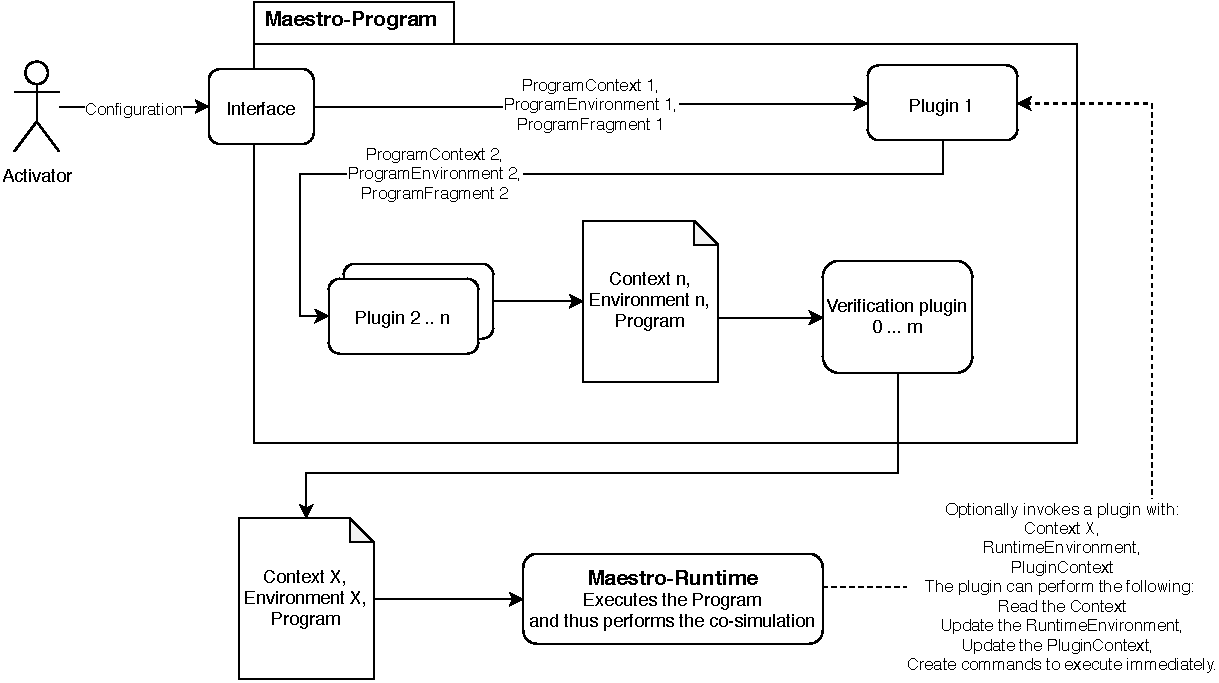
\includegraphics[width=\textwidth]{figures/conducting_co-simulation_overview.pdf}
  \caption{Conducting a co-simulation with Maestro-Program and Maestro-Runtime}
  \label{fig:conducting_co-simulation-overview}
\end{figure}

The following paragraphs describes the content of the figure. Initially, some
terminology and definitions are presented followed by a description of the
consecutive behavior.
\begin{description}
  \item[Context] Context is data and information related to the co-simulation.
    For example, the FMUs to employ in a given co-simulation or the dependencies
    between the variables of the FMUs for a given co-simulation.
  \item[Environment] The environment is information related to variables. For
    example, type information or the value of a given variable.
  \item[ProgramContext] Terminology for the Context used in relation to
    Maestro-Program.
  \item[ProgramEnvironment] Terminology for the Environment used in relation to
    Maestro-Program.
  \item[RuntimeContext] Terminology for Context used in relation to
    Maestro-Runtime.
  \item[RuntimeEnvironment] Terminology for the Environment used in relation to
    Maestro-Runtime. This contains i.e. variables in scope and values of variables.
  \item[PluginContext] A plugin specific Context. Maestro-Runtime does not know
    its content and the code to process it must be provided by the respective
    plugin.
    \item[Configuration] Configuration describing how to create the Program,
    i.e. which FMUs and plugins to use.
  \item[Root Context] Terminology for the initial Program Context. Examples of
    data in the Root Context is i.e. FMUs to use in a
    co-simulation and parameters for the FMUs.
  \item[Program] A Program is a complete in the sense that it can be passed to
    Maestro-Runtime for execution as opposed to a ProgramFragment described below.
  \item[Program Fragment] A Program Fragment is part of a Program.
  \item[Plugin] During the Program phase a plugin can read/update the Program
    Fragment, and/or read/update the ProgramContext and/or read/update the
    ProgramEnvironment. An example of ProgramContext information that a plugin can
    add is the dependencies between the variables of the FMUs. An example of a
    Program Fragment that a plugin can create is the necessary commands to perform
    initialisation of the FMUs. During the Runtime phase a plugin can read/update
    the RuntimeEnvironment, read/update the PluginContext and/or create commands to
    be executed immediately.
\end{description}

The Activator in \cref{fig:conducting_co-simulation-overview} is the entity
(person or tool) that launches a co-simulation. The Activator shall provide a
Configuration. See TODO.

Maestro-Program invokes the plugins according to the configuration. This
is demonstrated in \cref{fig:conducting_co-simulation-overview} where Plugin 1
receives ProgramContext 1, ProgramEnvironment 1, ProgramFragment 1 and
creates: ProgramContext 2, ProgramEnvironment 2 and ProgramFragment 2. This is
then passed to Plugin 2 and so on until no more plugins are specified. At this
stage it is expected that a Program has been created. It is then possible to
verify the Program, which is also based on plugins. The verification plugins can
report their results but cannot update the Program, context or environment. The
result of the Program phase is:
A Program (Program in the figure), a Context (Context X in the figure) and an Environment (Environment X
in the figure)

Maestro-Runtime executes the Program and can utilise the related Context and Environment.
It is possibly to create commands in
the Program that prompts Maestro-Runtime to invoke a specific plugin. The plugin
will be invoked with the initial Context (Context X in the figure), the Runtime
Environment (RunTimeEnvironment in the figure) and a Context for the specific plugin (PluginContext in the figure).



\subsection{TO BE DONE}
\begin{itemize}

\end{itemize}

%%% Local Variables: %%% mode: latex %%% TeX-master: "../Maestro" %%% End:

\clearpage
\section{Features and Use Cases}\label{sec:features_use-cases}

\clearpage
\section{Approach to Conducting a Co-simulation}
\label{sec:approach}

\clearpage
\section{Maestro Base Language}
\label{sec:mabl}

\clearpage
\section{Plugins}
\label{sec:plugins}

\clearpage
\section{Examples}\label{sec:examples}

\clearpage
\section{Future Work}
\label{sec:future-work}


\clearpage
\section{Legacy Context}
The Context contains information available to Maestro-Program,
plugins and Maestro-Runtime. These entities can also add information to the
Context by creating a new Context.

\subsection{Context Structure}
This section describes the structure of the Root Context and thereby what is
supported natively. The reason for natively supporting some data is that it is
considered essential for FMI co-simulation.
First, the entries are presented with an overall description. Afterwards, the types
mentioned in the overall description are described. Note, that not all entries are populated
by Maestro-Program prior to employing plugins. Some of these entries will be
populated by plugins. TODO: Clearly describe which entries Maestro-Program
populates.
\paragraph{Overall Structure}
\begin{description}
  \item[RawFMUs] The raw FMU information. Perhaps from a UI. Type: Map[FmuKey, FmuPath]
  \item[RawInstances] The raw instance information. Perhaps from a UI. Type: Map[FmuKey, List[InstanceKey]]
  \item[RawConnections] The raw connections information. Perhaps from a UI.
    Type: Map[{FmuKey, FmuInstance, ScalarVariableName}, Set[{FmuKey, FmuInstance, ScalarVariableName}]]
  \item[RawParameters] The raw parameters information. Perhaps from a UI.
    Type: Map[ParameterKey, Value] and Map[FMU, Map[Instance,
    Map[ScalarVariableName, ParameterKey]]]
  \item[Parameters] Parsed parameter information. Map[ScalarVariableID]
  \item[FMUsWithInstances] Enriches RawFMUs with ModelDescription information
    and connects FMUs to their respective instances. Type: Map[Fmu, Set[Instance]]
  \item[Connections] The connections based on FMUsWithInstances and variables
    from the corresponding ModelDescription files. Type: Set[Connection]
  \item[SortedDependantVariables] An list that describes the order of setting
    and getting dependant scalar variables according to internal and external
    dependencies. Type: List[ScalarVariableID]
    \item[Custom] This entry can be used freely. Type: Map[CustomDataKey, Any].
\end{description}

\paragraph{Types}
\begin{description}
  \item[FmuKey] String: Unique identifier for a given FMU
  \item[FmuPath] URI: Location of the FMU
  \item[InstanceKey] String: Unique identifier for a given instance
  \item[ScalarVariableName] String: Name of a given scalar variable.
    TODO: Perhaps valuereference, perhaps both?
  \item[Fmu] Data Object with FmuKey, FmuPath, ModelDescription.
  \item[Instance] Data Object that consists of parent FMU and InstanceKey
  \item[ModelDescription] The parsed model description.
  \item[Connection] Data Object with from of type ScalarVariableID and to of type Set[ScalarVariableID]
  \item[ScalarVariableID] Data Object that consists of Instance and ScalarVariableValueReference
  \item[CustomDataKey] String: Unique identifier for some custom data.
  \item[Any] Represents the value associated with a CustomDataKey.
    TODO: Represent as Sum Type: Any (Any) | JSON (String) | Text (String) |
    Byte (Array[Byte]) | ?
\end{description}

%%% Local Variables:
%%% mode: latex
%%% TeX-master: "../Maestro"
%%% End:

\clearpage
\section{Legacy Introduction}\label{sec:legacy_intro}
The framework is divided into two main parts: Maestro-Program and
Maestro-Runtime. These entities and the flow of conducting a co-simulation using
MaestroV2 is depicted in \cref{fig:conducting_co-simulation-overview} and
described in this section.

\begin{description}
  \item[Maestro-Program] is the entity that controls the process of creating a
program. A Program specifies how to conduct a co-simulation and consists of
commands to be carried out by Maestro-Runtime. In order to create a Program,
Maestro-Program employs plugins. The creation of a Program is referred to as the
Program Phase.
  \item[Maestro-Runtime] is the entity that controls the process of executing a
program. The execution of a program is referred to as the Execution Phase.

\end{description}
\begin{figure}[htb] \centering
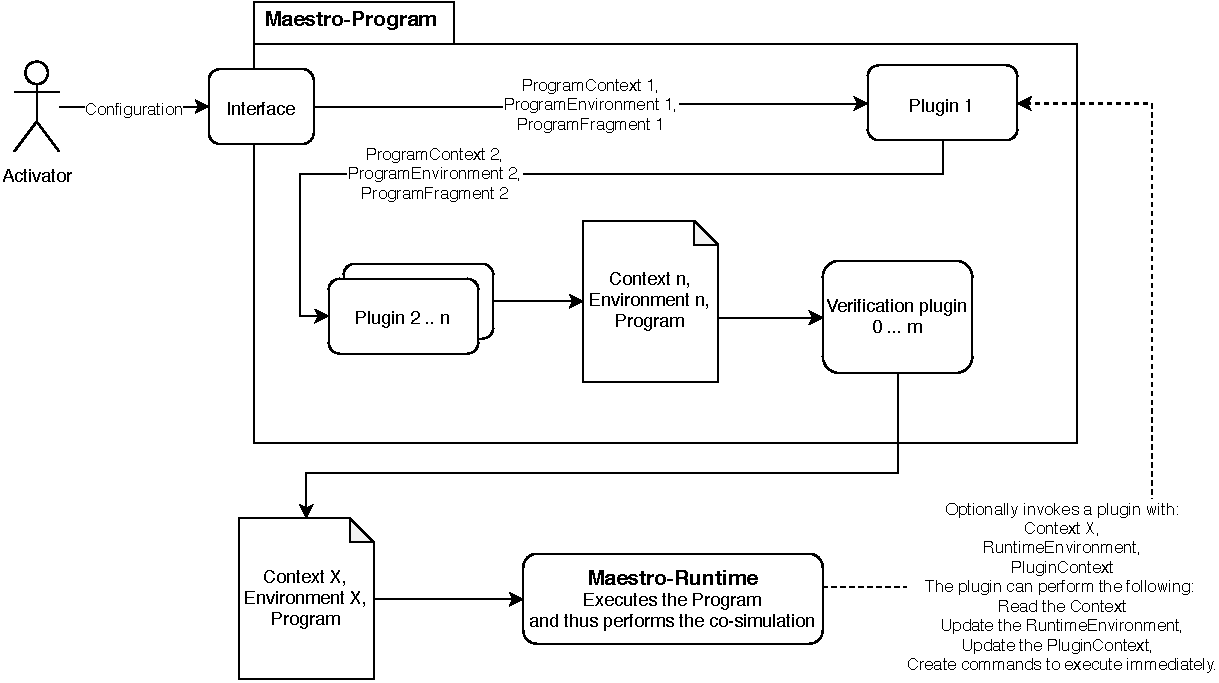
\includegraphics[width=\textwidth]{figures/conducting_co-simulation_overview.pdf}
  \caption{Conducting a co-simulation with Maestro-Program and Maestro-Runtime}
  \label{fig:conducting_co-simulation-overview}
\end{figure}

The following paragraphs describes the content of the figure. Initially, some
terminology and definitions are presented followed by a description of the
consecutive behavior.
\begin{description}
  \item[Context] Context is data and information related to the co-simulation.
For example, the FMUs to employ in a given co-simulation or the dependencies
between the variables of the FMUs for a given co-simulation.
  \item[Environment] The environment is information related to variables. For
example, type information or the value of a given variable.
  \item[ProgramContext] Terminology for the Context used in relation to
Maestro-Program.
  \item[ProgramEnvironment] Terminology for the Environment used in relation to
Maestro-Program.
  \item[RuntimeContext] Terminology for Context used in relation to
Maestro-Runtime.
  \item[RuntimeEnvironment] Terminology for the Environment used in relation to
Maestro-Runtime. This contains i.e. variables in scope and values of variables.
  \item[PluginContext] A plugin specific Context. Maestro-Runtime does not know
its content and the code to process it must be provided by the respective
plugin.
  \item[Configuration] Configuration describing how to create the Program, i.e.
which FMUs and plugins to use.
  \item[Root Context] Terminology for the initial Program Context. Examples of
data in the Root Context is i.e. FMUs to use in a co-simulation and parameters
for the FMUs.
  \item[Program] A Program is a complete in the sense that it can be passed to
Maestro-Runtime for execution as opposed to a ProgramFragment described below.
  \item[Program Fragment] A Program Fragment is part of a Program.
  \item[Plugin] During the Program phase a plugin can read/update the Program
Fragment, and/or read/update the ProgramContext and/or read/update the
ProgramEnvironment. An example of ProgramContext information that a plugin can
add is the dependencies between the variables of the FMUs. An example of a
Program Fragment that a plugin can create is the necessary commands to perform
initialisation of the FMUs. During the Runtime phase a plugin can read/update
the RuntimeEnvironment, read/update the PluginContext and/or create commands to
be executed immediately.
\end{description}

The Activator in \cref{fig:conducting_co-simulation-overview} is the entity
(person or tool) that launches a co-simulation. The Activator shall provide a
Configuration. See TODO.

Maestro-Program invokes the plugins according to the configuration. This is
demonstrated in \cref{fig:conducting_co-simulation-overview} where Plugin 1
receives ProgramContext 1, ProgramEnvironment 1, ProgramFragment 1 and creates:
ProgramContext 2, ProgramEnvironment 2 and ProgramFragment 2. This is then
passed to Plugin 2 and so on until no more plugins are specified. At this stage
it is expected that a Program has been created. It is then possible to verify
the Program, which is also based on plugins. The verification plugins can report
their results but cannot update the Program, context or environment. The result
of the Program phase is: A Program (Program in the figure), a Context (Context X
in the figure) and an Environment (Environment X in the figure)

Maestro-Runtime executes the Program and can utilise the related Context and
Environment. It is possibly to create commands in the Program that prompts
Maestro-Runtime to invoke a specific plugin. The plugin will be invoked with the
initial Context (Context X in the figure), the Runtime Environment
(RunTimeEnvironment in the figure) and a Context for the specific plugin
(PluginContext in the figure).



\subsection{TO BE DONE}
\begin{itemize}

\end{itemize}


%%% Local Variables:
%%% mode: latex
%%% TeX-master: "../Maestro"
%%% End:

\clearpage
%
%
%
%
%%%% Bibliography %%%%
\bibliographystyle{alpha}
\bibliography{bibliography}
\label{ch:bib} %label to refer to
%
%
%
\clearpage
%
%
%
\appendix
\section{List of Acronyms}\label{appendix:acronyms}
\begin{longtable}{ll}
XML	&Extensible Markup Language\\
\end{longtable}

\clearpage
%
%
%
\end{document}

%%% Local Variables:
%%% mode: latex
%%% TeX-master: t
%%% End:
